% !TEX root = ../main.tex


\section{Description of Sample Application}
\todo{Karla: Modify figures and change text accordingly}
To illustrate the development and analysis process of a design using the previously described 
statechart semantics, we will discuss a quadrotor helicopter or quadrotor application similar to 
the one presented by Syriani et al.~\cite{Syriani_2019}. The application will focus on the incremental 
design of some of the drone's required functionality.
The model constructed must obey statechart refinement rules that are proven within the Rodin tool.
The structure of the statechart for this model at each subsequent abstraction level restrict farther 
development of the model to refinements that obey the rules. This will allow us to prove properties 
of the model in a very strategic fashion, as properties proven of early abstraction levels 
are preserved in later refinements.

The first abstraction of the model shown in figure~\ref{fig:drone1} captures the basic 
functionality of the drone. The model initial state is |OFF| and as a result of the |on| and 
|toTakeoff| external triggers it transitions to the |START| and |OPERATIONAL| states respectively. 
The drone reacts to the |off| external trigger by shutting down and subsequently transitioning to the |OFF| state.
Within the |OPERATIONAL| state the drone will transition to |FLY|, |DESCEND| or |LANDED| 
after the internal triggers |toFly|, |toLand| or |landed| respectively. 
In this abstraction, these internal triggers are raised non-deterministically 
in the system by functionality not currently defined.
As additional details are incorporated into the model in later refinements some of that non-determinism is 
removed and replaced by transitions with actions that raised the previously defined internal triggers.

\begin{figure}[!h]
	\vspace{-.4cm}
	\centering
	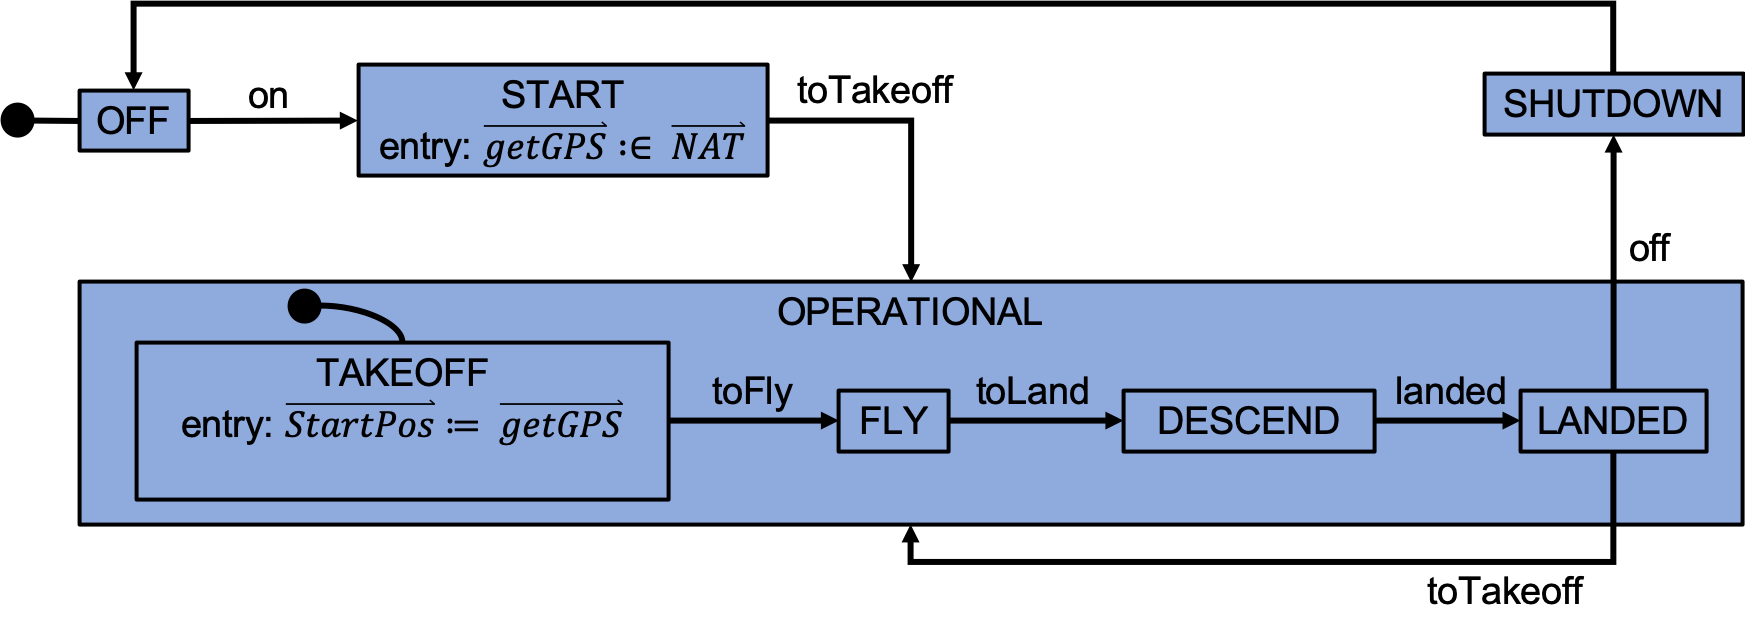
\includegraphics[width=0.95\textwidth]{figures/Picture1.png}
	\caption{Statechart of drone application. Abstract level including only generic behavior }
	\label{fig:drone1}
	\vspace{-.4cm}
\end{figure} 

% Figure~\ref{fig:drone4} shows three subsequesnt refinements to the drone model.
% The first refinement of the model, as we refine the parent state |TAKEOFF|
Figure~\ref{fig:drone2} shows the first refinement of the model, as we refine the parent state |TAKEOFF|
by introducing child states and new model variables, similar to the rule 1 and 2 defined by Syriani et al.
As part of this refinement we introduced an untriggered transition responsible for 
raising the |toFly| internal trigger, and therefore removed some of the non-determinisms in the abstraction.

\begin{figure}[!h]
	\centering
	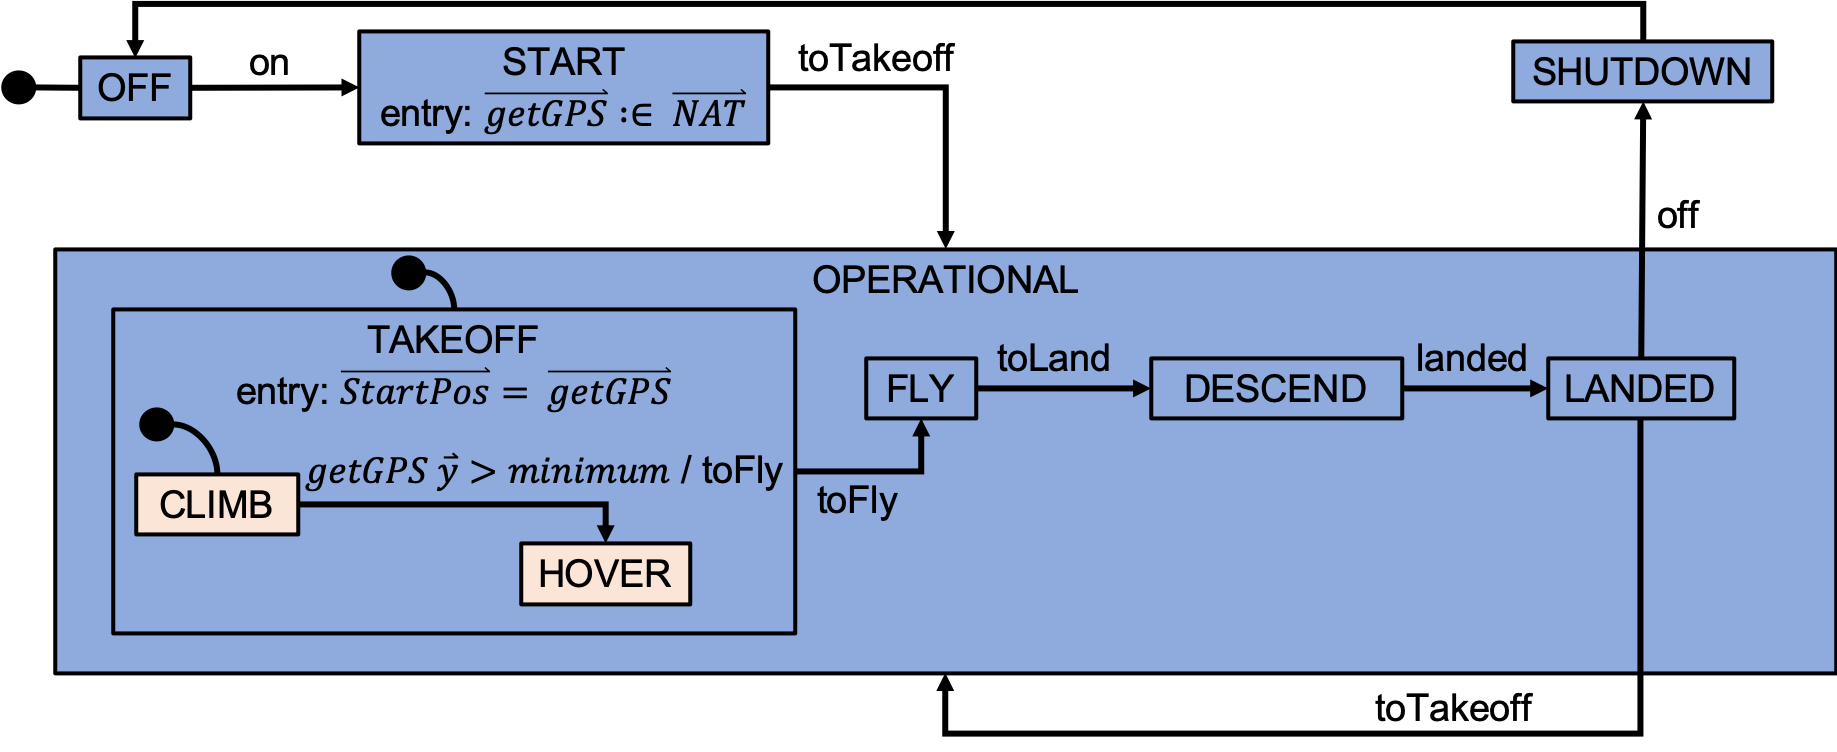
\includegraphics[width=0.95\textwidth]{figures/Picture2.png}
	\caption{Statechart of drone application. Refinement level introducing details for TakeOff}
	\label{fig:drone2}
\end{figure} 

\begin{figure}[!h]
	\centering
	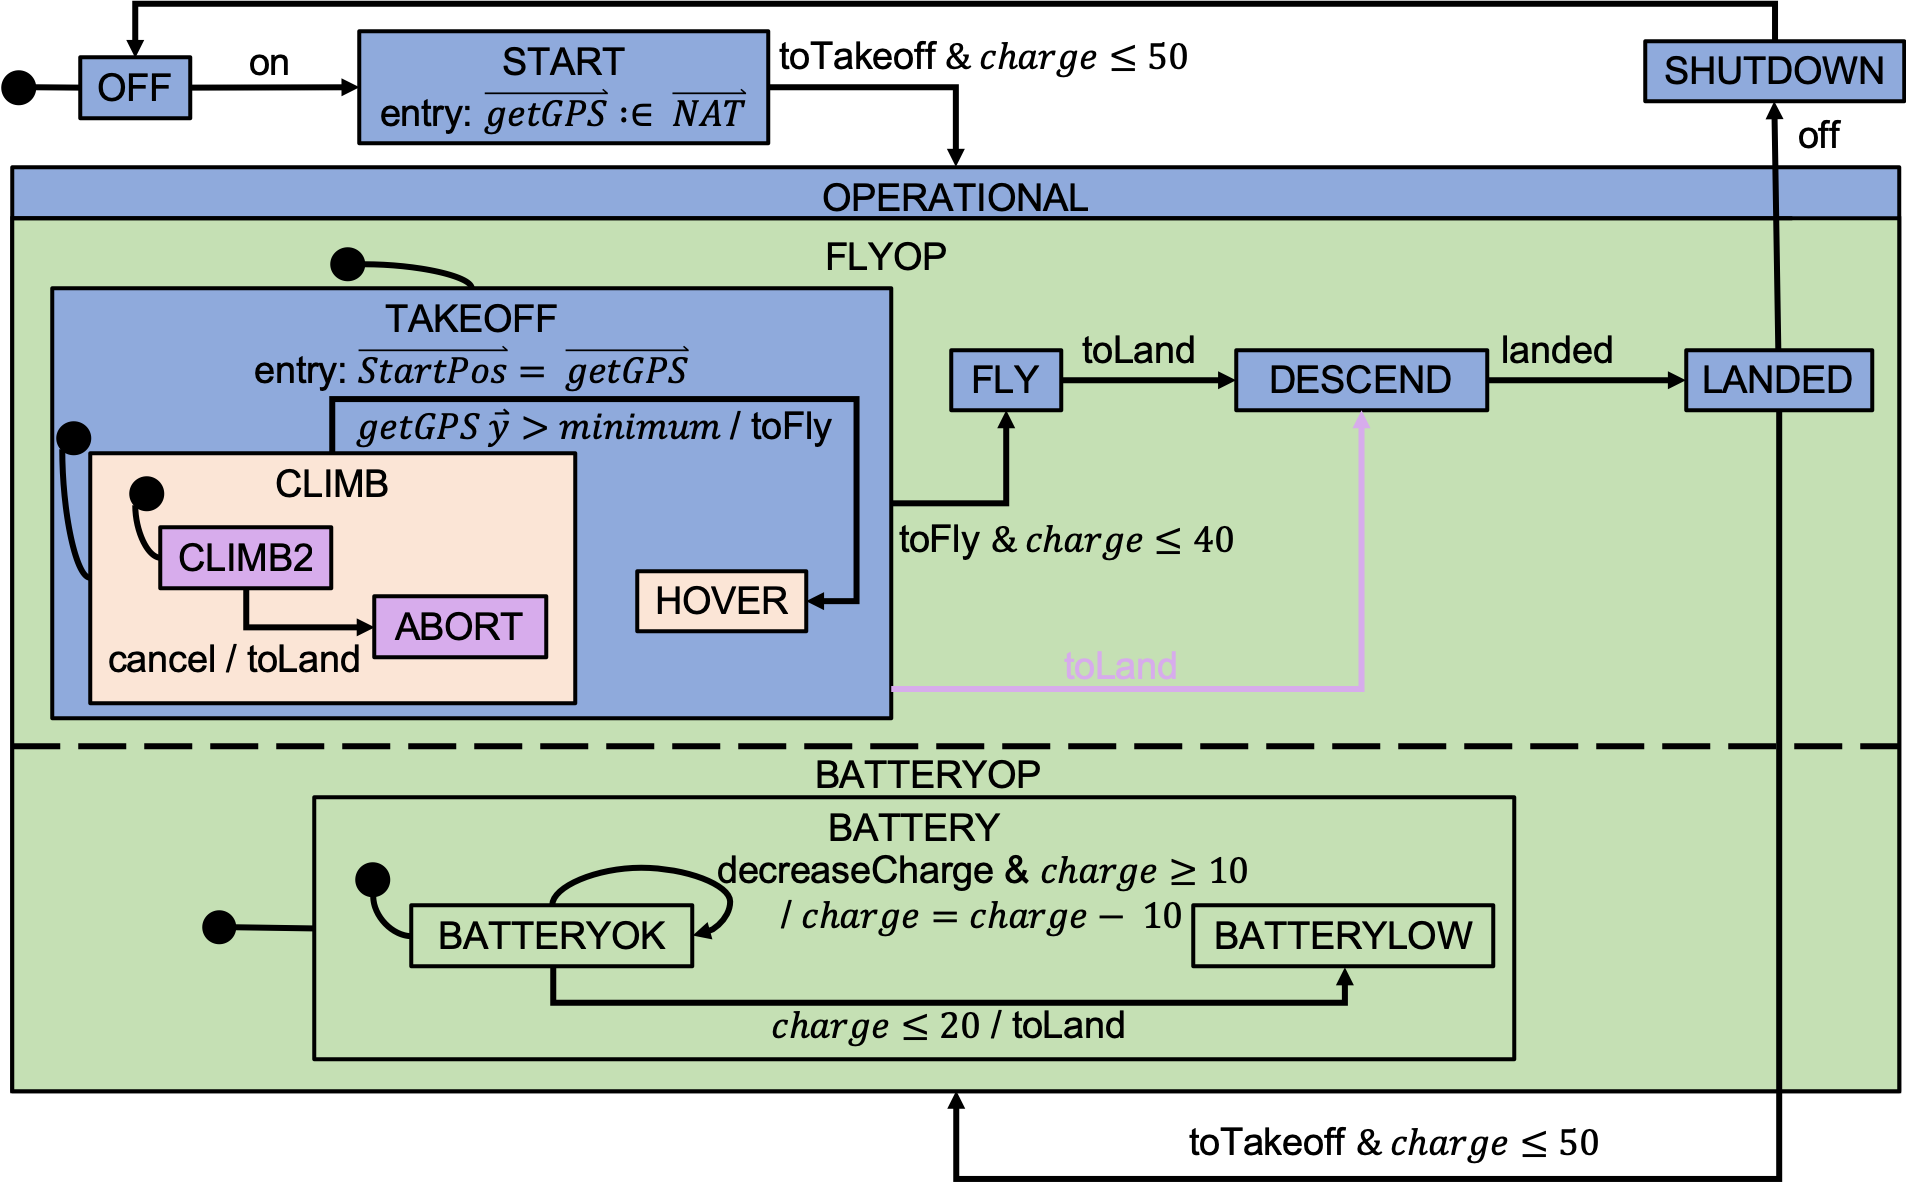
\includegraphics[width=0.95\textwidth]{figures/Picture5.png}
	\caption{Statechart of drone application. Refinement level for battery consumption functionality}
	\label{fig:drone4}
\end{figure} 

% The second refinement, figure~\ref{fig:drone3} extends the capabilities within |OPERATIONAL| by making it a parallel
Figure~\ref{fig:drone4} shows two subsequesnt refinements to the drone model.
The second refinement, the details of which are shown in green in figure~\ref{fig:drone4}, 
extends the capabilities within |OPERATIONAL| by making it a parallel
state that controls flying and battery related functionality. This is same as rule 4 defined by Syriani et al.
The charge within the drone battery is control by the parallel |BATTERYOP| state. 
The functionality is modeled by introducing a new model variable |charge|, which is decreased as 
a response to the internal trigger |decreaseCharge|. The aforementioned trigger, is raised non-deterministic by some 
unspecified internal functionality. Our statechart semantics support transition refinement, as such
we are able to modified preciously defined transitions. In particular, this type of refinement allow
us to add guards and/or actions to previously defined transitions. These new strengthening of guards, or additional 
actions are expression in term on new model variables that contribute implementation details to the model.
To ensure the drone operates with enough battery power we strengthen the guards of transitions to |FLY| and |TAKEOFF|.
As part of this design stage we introduce a requirement to constrain drone operation to battery charge of 
at least 20\% of its capacity. This can be expressed as |(BATTERYOK = TRUE) => charge > 20|\%

% \begin{figure}[!h]
% 	\centering
% 	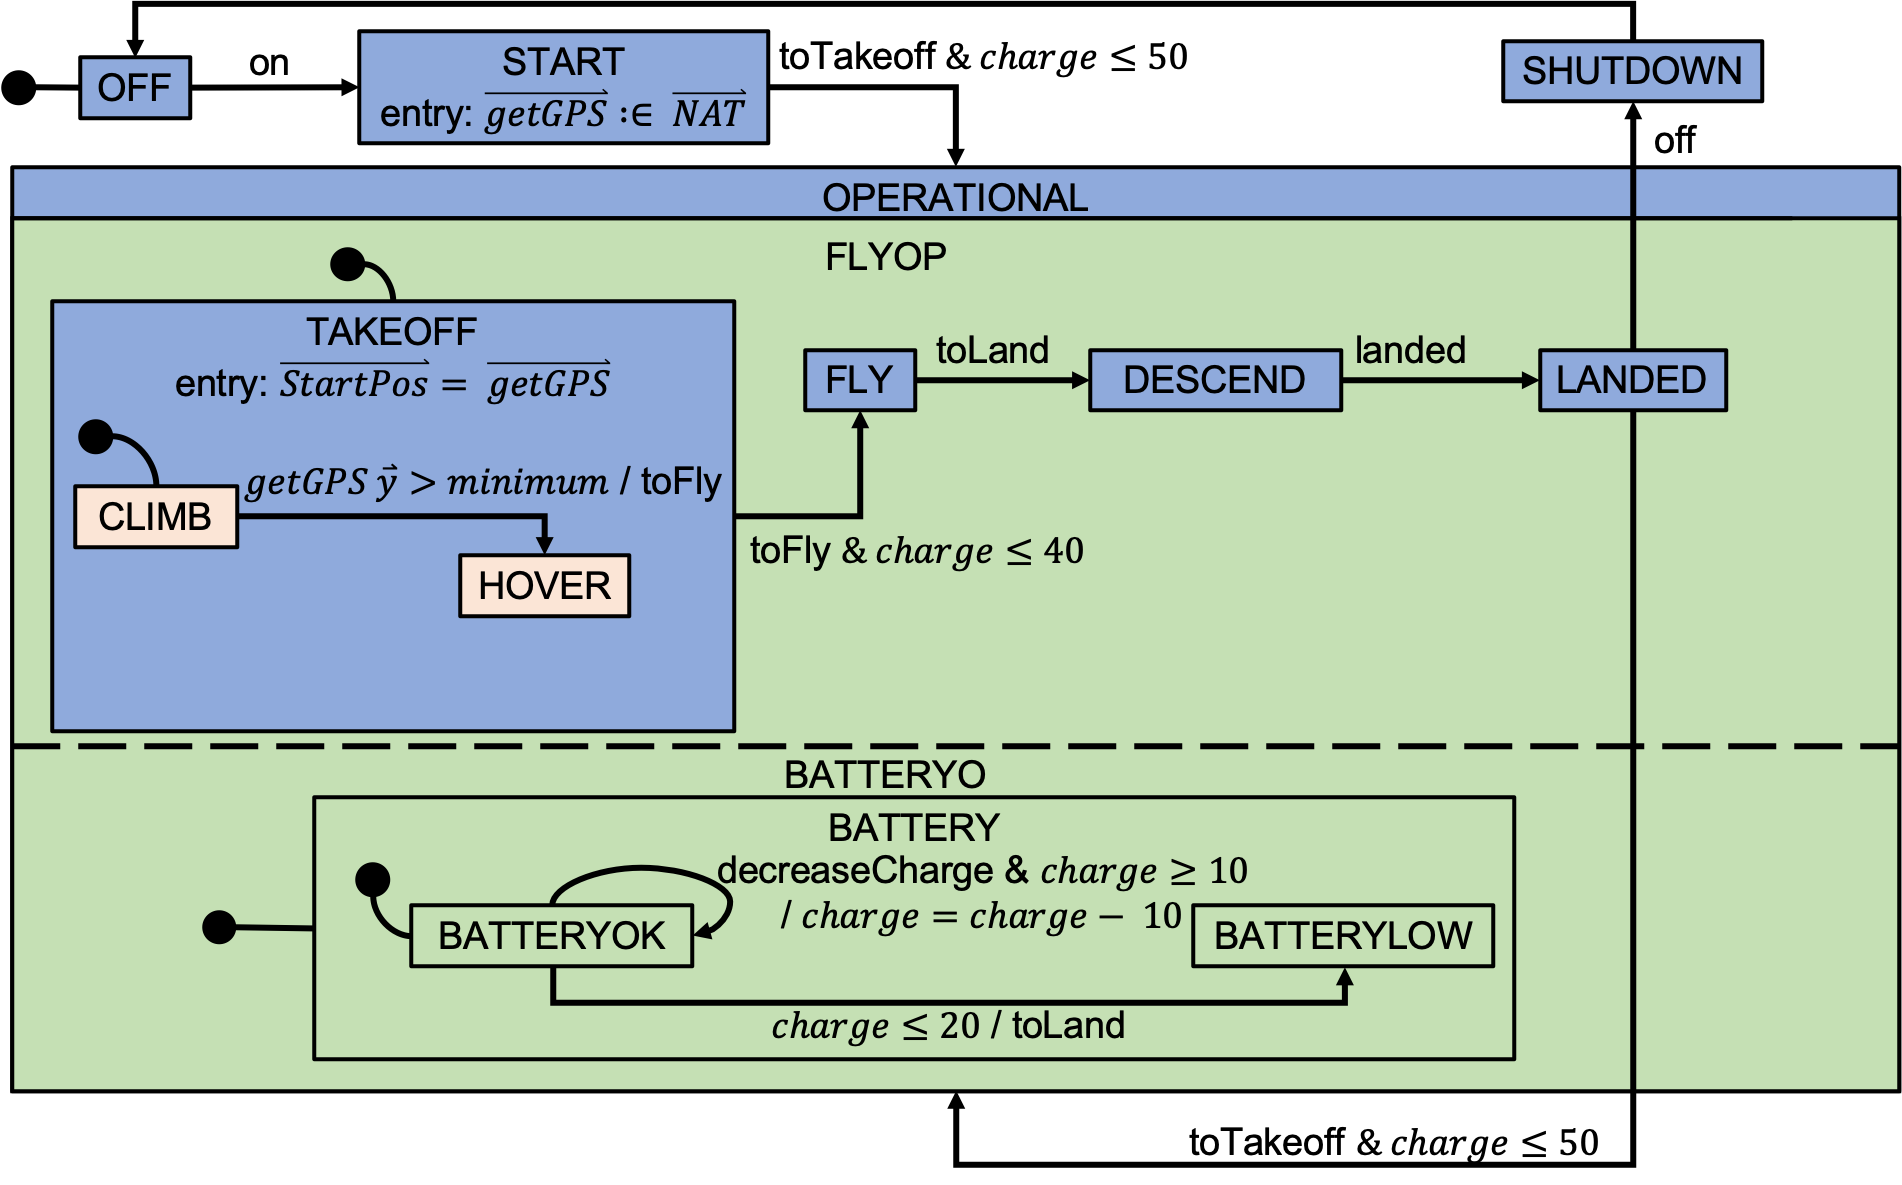
\includegraphics[width=0.95\textwidth]{figures/Picture3.png}
% 	\caption{Statechart of drone application.Refinement level for descending capabilities}
% 	\label{fig:drone3}
% \end{figure} 

% Figure~\ref{fig:drone4} shows a third refinement of the drone model, 
Figure~\ref{fig:drone4} shows a third refinement of the drone model, with features added in lilac.
At this stage we introduce additional implementation details to ensure that under special 
circumstances (e.g sensing of adverse environment or unexpected battery dropped) the drone is able 
to circumvent flying and proceed to an emergency landing. The previously described requirement can be
expressed as |(TAKEOFF = TRUE) => (BATTERYOK = TRUE ∨ toLand)|.
% \emph{What should be the expression for this property the invariant on line 84 seems strange to me}
To implement this new capability in the design we internal trigger |cancel| is introduced.
The internal trigger |cancel| can be raise non-deterministically by some sensing capability, 
the details of which are not currently implemented. If the trigger is raised the climbing process 
must be aborted and the drone descending sequence shall start. The ability to abort the 
takeoff operation and perform an emergency descend was not included on 
any of the previously outlined abstractions (see figures~\ref{fig:drone1} -~\ref{fig:drone2}) 


